% !TEX program = xelatex
% ---------------------------------------------------------------------------
%  Ὁ Πενταμετρικὸς Κύκλος — The Pentametric Cycle
%  Compile with:  latexmk -xelatex pentametric_cycle.tex   (or xelatex twice)
%  Requires the figure files fig1_spiral.pdf, fig2_area.pdf, fig3_palindrome.pdf
% ---------------------------------------------------------------------------
\documentclass[11pt,a4paper]{article}

\usepackage[margin=2.6cm]{geometry}
\usepackage{amsmath,amsthm,mathtools}
\usepackage{fontspec}
\usepackage{unicode-math}
\setmainfont{Latin Modern Roman}
\setmathfont{Latin Modern Math}
\newfontfamily\greekfont{GFS Porson}[Scale=MatchLowercase,ItalicFont={GFS Porson},BoldFont={GFS Porson},BoldFeatures={FakeBold=2}]
\newfontfamily\symbolfont{DejaVu Sans}
\usepackage{graphicx}
\usepackage{booktabs,array,longtable,tabularx}
\usepackage{enumitem}
\usepackage[edges]{forest}
\usepackage{xcolor}
\usepackage[hidelinks]{hyperref}
\usepackage{titlesec}
\usepackage{caption}
\usepackage[most]{tcolorbox}
\captionsetup{font=small,labelfont=bf}

% ---- notation --------------------------------------------------------------
\newcommand{\gr}[1]{{\greekfont #1}}                 % polytonic Greek
\newcommand{\Pent}{\mathfrak{P}}                      % the Pentametric Formula
\newcommand{\note}{\text{\symbolfont ♪}}              % musical annotation
\newcommand{\leg}[1]{\left(\tfrac{#1}{5}\right)}      % Legendre symbol mod 5
\newcommand{\Z}{\mathbb{Z}}

% ---- theorem environments --------------------------------------------------
\theoremstyle{plain}
\newtheorem{theorem}{Theorem}[section]
\newtheorem{proposition}[theorem]{Proposition}
\newtheorem{lemma}[theorem]{Lemma}
\newtheorem{corollary}[theorem]{Corollary}
\theoremstyle{definition}
\newtheorem{definition}[theorem]{Definition}
\theoremstyle{remark}
\newtheorem{remark}[theorem]{Remark}
\newtheorem*{interp}{Interpretive remark}

\hypersetup{
  pdftitle={The Pentametric Cycle},
  pdfauthor={Lluis Garcia Torcal},
  pdfkeywords={Fibonacci numbers, Lucas numbers, Legendre symbol, palindromic sequences, Fibonacci tiling, Pythagorean consonances}
}

\begin{document}

% =============================================================================
%  TITLE PAGE
% =============================================================================
\begin{titlepage}
\centering
\vspace*{2.2cm}
{\fontsize{30}{36}\selectfont \gr{Ὁ Πενταμετρικὸς Κύκλος}\par}
\vspace{0.6cm}
{\Large A Nested Palindrome Encoding the Pythagorean Consonances\par}
\vspace{0.3cm}
{\large\itshape (The Pentametric Cycle)\par}
\vspace{1.6cm}
{\fontsize{40}{48}\selectfont $\Pent(n)$\qquad $\note(n)$\par}
\vspace{1.4cm}
\begin{minipage}{0.78\textwidth}\centering\small
$\displaystyle \Pent(n)=\frac{n^{2}+4\,C(m)}{5},\qquad m=4n^{2}\bmod 10,\qquad C(m)=\frac{26m-5m^{2}}{24}$
\\[0.8em]
$\displaystyle \Pent(L_k)=F_k^{2}$
\end{minipage}
\vfill
{\large Lluis Garcia Torcal\par}
\vspace{0.2cm}
{Independent researcher\par}
\vspace{0.2cm}
{October 2026\par}
\vspace{1.2cm}
{\small Manuscript submitted for peer review}
\end{titlepage}

% =============================================================================
%  ABSTRACT
% =============================================================================
\begin{abstract}
\noindent
We present the \emph{Pentametric Cycle} (\gr{Ὁ Πενταμετρικὸς Κύκλος}), a structure generated by an integer-valued quadratic formula $\Pent(n)$, the \emph{Pentametric Formula}. We show that the formula's correction term, an interpolating polynomial $C(m)$ called the \emph{Interval Map}, coincides on every attained residue with the Legendre symbol $\leg{n}$, so that $\Pent(n)=\bigl(n^{2}+4\leg{n}\bigr)/5$. We collect ten equivalent forms of $\Pent$ found by the author. They use decimal digits, floors, a quintic polynomial, cosines (a quadratic Gauss sum), rotations by the golden ratio and pentagonal angles. We prove that each one computes the same quadratic character, and we derive the general laws $\Pent(n)-n^{2}/5=\pm\tfrac45$ and $\pm\tfrac{2\pi}{5}$ for square and circle areas. Reducing the doubled value $2\Pent(n)$ modulo~$10$ and halving gives a digit $H(n)\in\{0,1,2,3,4\}$; the single rule $H:(H-1)$ then turns it into silence or one of the four Pythagorean consonances (unison, octave, fifth, fourth). The sequence $H$ has minimal period $25=5^{2}$ and is even, so its restrictions to $n=0,\dots,25$ and $n=0,\dots,50$ are palindromes. In each period, $9=3^{2}$ terms are silent and the four consonances occur exactly $4$ times each, $16=4^{2}$ in all; we read this split interpretively against the triple $3^{2}+4^{2}=5^{2}$. We prove the \emph{Pentametric–Lucas Theorem}: $\Pent(L_k)=F_k^{2}$ for every Lucas number $L_k$. We also prove its converse: for $n\ge 1$, $\Pent(n)$ is a perfect square if and only if $n$ is a Lucas number. We confirm the author's conjecture that the areas at Lucas positions admit a form as simple as the distances: $F_k=\operatorname{round}(L_k\sqrt{0.2})$ for $k\ge2$. Finally, we relate the theorem to the classical result of Holden (1975), according to which the centres of spiralling Fibonacci squares lie on two orthogonal lines at distances $L_k/\sqrt{10}$ from their intersection. We call this the \emph{Geometric Lucas Meter} and fully credit it to Holden. We derive from it two new geometric identities that make $\Pent$ visible in the Fibonacci tiling: a difference of $\pm\tfrac45$ in square areas and of $\pm\tfrac{2\pi}{5}$ in circle areas.
\end{abstract}

\medskip
\noindent\textbf{Keywords:} Fibonacci numbers; Lucas numbers; Legendre symbol; palindromic sequences; Fibonacci tiling; Pythagorean consonances.

\noindent\textbf{MSC 2020:} 11B39 (primary); 11A07, 11B50, 51M04, 00A65 (secondary).

\newpage
\tableofcontents

\vspace{1.2em}
\begin{tcolorbox}[enhanced,colback=black!3,colframe=black!55,boxrule=0.5pt,arc=1pt,left=8pt,right=8pt,top=5pt,bottom=5pt,title={\textbf{Main results at a glance}},coltitle=black,colbacktitle=black!10,fonttitle=\small]
\small
\begin{itemize}[leftmargin=1.2em,itemsep=1.5pt,topsep=1pt]
  \item \textbf{Closed form.} $\Pent(n)=\bigl(n^{2}+4\leg{n}\bigr)/5$; the Interval Map $C(m)$ is the Legendre symbol on attained residues (Lemma~\ref{lem:legendre}).
  \item \textbf{The Pentametric family.} Ten equivalent forms of $\Pent$ via digits, floors, a quintic, a Gauss sum, golden rotations and pentagonal angles (Proposition~\ref{prop:selectors}, Theorem~\ref{thm:family}).
  \item \textbf{The $\pm0.8$ and $\pm2\pi/5$ laws} for every $n$ (Proposition~\ref{prop:defects}); palindromic last digits of period $50$ (Proposition~\ref{prop:lastdigits}).
  \item \textbf{Derivation of the ratios.} A seven-step deterministic chain $n\mapsto m\mapsto C(m)\mapsto\Pent(n)\mapsto 2\Pent(n)\mapsto H\mapsto\rho(H)$ (§\ref{sec:derivation}).
  \item \textbf{Vertebra and Palindrome.} Period $25$; $9$ silences and $4$ of each consonance; $51$-term palindrome mirrored at $n=25$ (Propositions~\ref{prop:period}, \ref{prop:counts}, \ref{prop:palindrome}).
  \item \textbf{Pentametric–Lucas Theorem} $\Pent(L_k)=F_k^{2}$ and its \textbf{converse}: squares occur only at Lucas numbers (Theorems~\ref{thm:PL}, \ref{thm:converse}).
  \item \textbf{The author's conjecture confirmed:} $F_k=\operatorname{round}(L_k\sqrt{0.2})$, mirroring the distance $L_k\sqrt{0.1}$ (Proposition~\ref{prop:simple}).
  \item \textbf{Geometric Lucas Meter} (Holden, 1975; Theorem~\ref{thm:holden}) and its link to $\Pent$: square/circle identities and the $3$–$4$–$5$ angles (Propositions~\ref{prop:geom}, \ref{prop:angles}).
\end{itemize}
\end{tcolorbox}

\vspace{0.8em}
\begin{center}
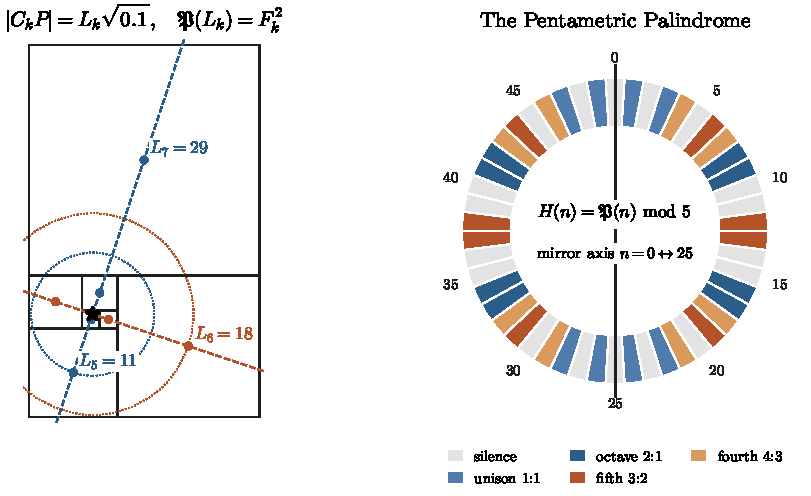
\includegraphics[width=0.92\textwidth]{fig0_abstract.pdf}
\captionof{figure}{Graphical abstract. Left: the Fibonacci squares, Holden's orthogonal lines and their intersection $P$ (star); the centre of the $k$-th square lies at distance $L_k\sqrt{0.1}$ from $P$ (dotted circles for $k=5,6$), and $\Pent(L_k)=F_k^{2}$ is its area. Right: one period ($n=0,\dots,49$) of the consonance sequence $H(n)$, mirrored across the axis through $n=0$ and $n=25$.}\label{fig:abstract}
\end{center}
\newpage

% =============================================================================
\section{Introduction}\label{sec:intro}
% =============================================================================

The Pythagorean tradition sought to express musical harmony through number. The consonances were understood as ratios: unison ($1:1$), octave ($2:1$, \gr{διὰ πασῶν}), fifth ($3:2$, \gr{διὰ πέντε}) and fourth ($4:3$, \gr{διὰ τεσσάρων}). The monochord (\gr{κανών}) was the instrument for measuring them \cite{Barker1989,Levin1994,Bower1989}. All four ratios are built from the numbers $1,2,3,4$ of the \emph{tetractys}. This paper studies an integer sequence whose reduced values fall into exactly five classes, which we read as silence and these four consonances.

The structure emerged from the study of square areas generated by a quadratic expression in $n$, worked out by the author with dynamic-geometry constructions (GeoGebra) and spreadsheet experiments. The resulting formula $\Pent(n)$, the \emph{Pentametric Formula}, always produces an integer. When its value is doubled and reduced modulo~$10$, only five residues remain. The resulting sequence is periodic and palindromic, and its counts follow the pattern $9+16=25$.

The formula also connects to a classical geometric fact. In 1975, H.\,L.~Holden showed that the centres of the squares in the Fibonacci spiral lie on two perpendicular lines, and that their distances from the intersection point are proportional to the Lucas numbers \cite{Holden1975}. The result was extended by Hoggatt and Alladi \cite{HoggattAlladi1975} and later rediscovered in a classroom setting and published by Gardiner \cite{Gardiner1984}. We show that the Lucas numbers which locate these centres are exactly the arguments at which $\Pent$ returns the areas of the corresponding squares.

\paragraph{Contributions.} We separate clearly what is classical from what is claimed as new.
\begin{enumerate}[label=(\roman*),itemsep=2pt]
  \item \emph{Classical (cited, not claimed):} the identity $L_k^{2}-5F_k^{2}=4(-1)^{k}$ \cite{Koshy2001}; Gessel's characterisation of Fibonacci numbers \cite{Gessel1971}; the orthogonal-lines property of the centres of Fibonacci squares and the Lucas-number distances \cite{Holden1975,HoggattAlladi1975,Gardiner1984}.
  \item \emph{New (this paper):} the Pentametric Formula and its nomenclature (§\ref{sec:defs}); the closed form via the Legendre symbol (Lemma~\ref{lem:legendre}); the family of ten equivalent forms of $\Pent$ and its side lengths, with the general $\pm0.8$ and $\pm2\pi/5$ laws and the palindromic last-digit sequences (§\ref{sec:family}); the author's conjecture on a simple form of the areas at Lucas positions, with its confirmation (§\ref{sec:conjecture}); the periodicity, palindromicity and counting results for $H$ (§§\ref{sec:doubling}–\ref{sec:counts}); the Pentametric–Lucas Theorem and its converse, with complete proofs (§\ref{sec:lucas}); the area and circle identities linking $\Pent$ to the Fibonacci tiling (§\ref{sec:geom-new}); and the musical reading (§\ref{sec:music}).
\end{enumerate}
Throughout, results that are proved are stated as theorems, propositions or lemmas. Numerological and musical readings are marked as \emph{interpretive remarks}. They do not form part of the mathematical claims.

\paragraph{Conventions.} $F_0=0,\ F_1=1,\ F_{k+1}=F_k+F_{k-1}$; $L_0=2,\ L_1=1,\ L_{k+1}=L_k+L_{k-1}$. For an integer $n$, $\leg{n}$ is the Legendre symbol modulo $5$: it equals $0$ if $5\mid n$, $+1$ if $n\equiv\pm1\pmod 5$, and $-1$ if $n\equiv\pm2\pmod 5$.

% =============================================================================
\section{Definitions and notation}\label{sec:defs}
% =============================================================================

\subsection{The Pentametric Formula}

\begin{definition}[The Pentametric Formula, \gr{Ὁ Πενταμετρικὸς Τύπος}]\label{def:P}
For $n\in\Z_{\ge0}$ put
\begin{equation}\label{eq:P}
  \Pent(n)=\frac{n^{2}+4\,C(m)}{5},\qquad m=4n^{2}\bmod 10,\qquad C(m)=\frac{26m-5m^{2}}{24}.
\end{equation}
The symbol $\Pent$ (fraktur P) stands for \emph{Pentametric} and is read “the Pentametric of $n$”. Formula \eqref{eq:P} is one of several equivalent forms found by the author. Lemma~\ref{lem:legendre} gives a canonical one, and §\ref{sec:family} collects the whole family.
\end{definition}

\subsection{Supporting notation}

\begin{center}
\begin{tabular}{@{}ll@{}}
\toprule
Symbol & Meaning \\
\midrule
$\Pent(n)$ & the Pentametric area \\
$\sqrt{\Pent(n)}$ & the side length \\
$\Pent(n)\bmod 10$ & the area's last digit \\
$2\Pent(n)$ & the doubled area (Diapason, §\ref{sec:doubling}) \\
$H(n)$ & the halved digit (consonance indicator) \\
$\note(n)$ & the musical annotation (interval interpretation of $H(n)$) \\
\bottomrule
\end{tabular}
\end{center}

\subsection{The Interval Map}

\begin{definition}[The Interval Map, \gr{Ὁ Διαστηματικὸς Χάρτης}; also the Harmonic Canon, \gr{Ὁ Ἁρμονικὸς Κανών}]
$C(m)=(26m-5m^{2})/24$ is the unique polynomial of degree at most two that interpolates the values
\begin{center}
\begin{tabular}{@{}cccccc@{}}
\toprule
$m$ & $0$ & $2$ & $4$ & $6$ & $8$\\
$C(m)$ & $0$ & $\tfrac43$ & $1$ & $-1$ & $-\tfrac{14}{3}$\\
\bottomrule
\end{tabular}
\end{center}
on the five even residues modulo~$10$.
\end{definition}

The following lemma shows that only three of these five values are ever reached. On those three, $C$ is a classical arithmetic function.

\begin{lemma}[Attained residues]\label{lem:legendre}
For every integer $n$, $m=4n^{2}\bmod 10\in\{0,4,6\}$, and
\[
  C(4n^{2}\bmod 10)=\leg{n}.
\]
Consequently
\begin{equation}\label{eq:closed}
  \boxed{\;\Pent(n)=\frac{n^{2}+4\leg{n}}{5}=\frac{n^{2}}{5}+\frac45\leg{n}\;}
\end{equation}
and $\Pent(n)$ is a non-negative integer for every $n\ge0$.
\end{lemma}

\begin{proof}
Squares modulo $10$ lie in $\{0,1,4,5,6,9\}$. Hence $4n^{2}\bmod 10$ is $0$ when $n^{2}\equiv0,5$; it is $4$ when $n^{2}\equiv1,6$; and it is $6$ when $n^{2}\equiv4,9\pmod{10}$. These three cases are exactly $5\mid n$, $n^{2}\equiv1\pmod5$ and $n^{2}\equiv4\pmod5$. In the same order, $\leg{n}$ equals $0,+1,-1$. Since $C(0)=0$, $C(4)=1$ and $C(6)=-1$, the identity follows. For integrality, $n^{2}+4\leg{n}\equiv 0,\ 1+4,\ 4-4\equiv0\pmod 5$ in the three cases. Non-negativity holds because $n^{2}\ge4$ whenever $\leg{n}=-1$.
\end{proof}

\begin{remark}
The values $C(2)=\tfrac43$ and $C(8)=-\tfrac{14}{3}$ are therefore never used by the Pentametric Formula. They are artefacts of the interpolation and carry no arithmetic meaning in $\Pent$. Equation \eqref{eq:closed} also answers the question of a general closed form for $\Pent(n)$ at arbitrary $n$. $\Pent(n)$ is the area $n^{2}/5$ of a square of side $n/\sqrt5=n\sqrt{0.2}$, shifted by exactly $\pm\tfrac45$ to an integer (by $0$ when $5\mid n$). This is the “$\pm0.8$” phenomenon observed in the author's GeoGebra constructions and spreadsheets. §\ref{sec:family} develops it, and §\ref{sec:geom-new} gives it a geometric meaning in the Fibonacci tiling.
\end{remark}


\subsection{The derivation of the ratios}\label{sec:derivation}

The ratios are not attached to the sequence position by position. They are produced by a fixed chain of operations, applied identically to every $n$. Given $n\in\Z_{\ge0}$:

\begin{center}
\renewcommand{\arraystretch}{1.25}
\begin{tabular}{@{}lll@{}}
\toprule
Step & Operation & Name \\
\midrule
1 & $m=4n^{2}\bmod 10$ & the residue \\
2 & $C(m)=(26m-5m^{2})/24$ & the Interval Map \\
3 & $\Pent(n)=\bigl(n^{2}+4C(m)\bigr)/5$ & the Pentametric area \\
4 & $2\Pent(n)$ & the Diapason doubling \\
5 & $2\Pent(n)\bmod 10$ & the last digit (always even) \\
6 & $H=\bigl(2\Pent(n)\bmod 10\bigr)/2\in\{0,1,2,3,4\}$ & the halved digit \\
7 & $\rho(H)=H:(H-1)$ for $H\ge2$;\ \ $\rho(1)=1:1$ & the ratio extraction \\
\bottomrule
\end{tabular}
\end{center}

\begin{definition}[Ratio extraction]\label{def:ratio}
The \emph{ratio extraction} $\rho$ assigns to each value of $H$ the ratio
\begin{center}
\begin{tabular}{@{}cccl@{}}
\toprule
$H$ & $\rho(H)$ & Interval & \\
\midrule
$0$ & — & silence & no ratio \\
$1$ & $1:1$ & unison & \\
$2$ & $2:1$ & octave & \\
$3$ & $3:2$ & fifth & \\
$4$ & $4:3$ & fourth & \\
\bottomrule
\end{tabular}
\end{center}
For $H\ge2$, $\rho(H)=H:(H-1)$ is the ratio of two consecutive members of the tetractys $1,2,3,4$. The value $H=1$ is set to the unison $1:1$, since $1:0$ is not a ratio.
\end{definition}

Once Definition~\ref{def:ratio} is fixed, the interval at position $n$ is a deterministic function of $n$:
\[
  n\ \longmapsto\ \rho\bigl(H(n)\bigr).
\]
No value is chosen case by case: Steps 1–6 are arithmetic identities, and Step~7 applies one rule uniformly to all $n$.

\begin{table}[ht]
\centering\small
\caption{Worked example of the derivation for $n=7$.}\label{tab:example7}
\renewcommand{\arraystretch}{1.25}
\begin{tabular}{@{}ll@{}}
\toprule
Step & Computation \\
\midrule
1 & $m=4\cdot7^{2}\bmod10=196\bmod10=6$ \\
2 & $C(6)=(26\cdot6-5\cdot6^{2})/24=(156-180)/24=-24/24=-1$ \\
3 & $\Pent(7)=\bigl(7^{2}+4\cdot(-1)\bigr)/5=(49-4)/5=45/5=9$ \\
4 & $2\Pent(7)=18$ \\
5 & $18\bmod10=8$ \\
6 & $H=8/2=4$ \\
7 & $\rho(4)=4:3$\quad (the fourth, \gr{διὰ τεσσάρων}) \\
\bottomrule
\end{tabular}
\end{table}

\noindent For $n=7$, therefore, the interval is the fourth ($4:3$), obtained entirely from the formula. The same chain applied to $n=0,\dots,50$ produces the Pentametric Palindrome of §\ref{sec:palindrome}.

\begin{remark}
In the terms of Lemma~\ref{lem:legendre}, Steps 1–3 compute $\Pent(n)=(n^{2}+4\leg{n})/5$, and Steps 4–6 compute $H(n)=\Pent(n)\bmod5$. Thus the arithmetic content of the chain is the pair $\bigl(n^{2}\bmod 25,\ \leg{n}\bigr)$, and $\rho\circ H$ is a function of $n\bmod 25$ (Proposition~\ref{prop:period}).
\end{remark}

% =============================================================================
\section{The family of Pentametric forms}\label{sec:family}
% =============================================================================

The author arrived at $\Pent$ through several independent spreadsheet constructions. Each one takes a different route to the same areas $\Pent(n)$ and side lengths $s(n)=\sqrt{\Pent(n)}$. This section collects them, gives each its proof, and shows that they all come down to a single fact: every form computes the quadratic character $\chi(n)=\leg{n}$ modulo~$5$ in a different way.

Throughout, write
\[
  \chi(n)=\leg{n},\qquad r=n^{2}\bmod 10,\qquad d=2n^{2}\bmod 10,\qquad m=4n^{2}\bmod 10 .
\]
As in the proof of Lemma~\ref{lem:legendre}, the three cases $5\mid n$, $n^{2}\equiv1$ and $n^{2}\equiv4\pmod 5$ give
\begin{center}
\begin{tabular}{@{}lcccc@{}}
\toprule
Case & $\chi(n)$ & $r$ & $d$ & $m$ \\
\midrule
$5\mid n$ & $0$ & $0,5$ & $0$ & $0$ \\
$n\equiv\pm1\pmod5$ & $+1$ & $1,6$ & $2$ & $4$ \\
$n\equiv\pm2\pmod5$ & $-1$ & $4,9$ & $8$ & $6$ \\
\bottomrule
\end{tabular}
\end{center}
The residue $d$ is also the first decimal digit of $n^{2}/5$, because $n^{2}/5$ has fractional part $0$, $0.2$ or $0.8$ in the three cases.

\subsection{Six ways to compute the correction}

\begin{proposition}[Selectors of the quadratic character]\label{prop:selectors}
Each of the following expressions equals $\chi(n)$ for every integer $n$.
\begin{enumerate}[label=(\roman*),itemsep=3pt]
  \item \emph{Interval Map in $m$:} $C(m)=\dfrac{26m-5m^{2}}{24}$.
  \item \emph{Double-square digit:} $\dfrac54\,p(d)$, where $p(d)=-\dfrac{d^{2}}{12}+\dfrac{17d}{30}$. Equivalently, $p(d)=\tfrac45\chi(n)\in\{0,+0.8,-0.8\}$.
  \item \emph{Square digit:} $\dfrac{x^{5}-35x^{3}+250x}{216}$, where $x=r-5$.
  \item \emph{Sign selector:} $T(d)=2g(d)-[\,d\neq0\,]$, where $g(d)=\dfrac{d(8-d)}{12}=\dfrac{8-d}{6}\cdot\dfrac d2$. Here $g(d)=1$ if $\chi(n)=+1$ and $g(d)=0$ otherwise. The Iverson bracket $[\,d\neq0\,]$ equals $1$ when $d\neq0$ and $0$ otherwise.
  \item \emph{Trigonometric (Gauss sum):} $\dfrac{2}{\sqrt5}\Bigl(\cos\dfrac{2\pi n}{5}-\cos\dfrac{4\pi n}{5}\Bigr)$.
  \item \emph{Pentagonal angle:} with $\alpha=72n\bmod 360$ (in degrees), the value $+1$ if $\alpha\in\{72,288\}$, $-1$ if $\alpha\in\{144,216\}$, and $0$ if $\alpha=0$.
\end{enumerate}
\end{proposition}

\begin{proof}
By the table above, each of (i)–(iv) is a function of a residue that takes only three values. It therefore suffices to evaluate each expression at those three values.
(i) $C(0)=0$, $C(4)=1$, $C(6)=-1$ (Lemma~\ref{lem:legendre}).
(ii) $p(0)=0$, $p(2)=-\tfrac13+\tfrac{17}{15}=\tfrac45$, $p(8)=-\tfrac{16}{3}+\tfrac{68}{15}=-\tfrac45$.
(iii) For $r\in\{0,1,4,5,6,9\}$ we have $x\in\{-5,-4,-1,0,1,4\}$. The odd quintic $q(x)=x^{5}-35x^{3}+250x$ takes the values $q(\pm5)=0$, $q(0)=0$, $q(1)=216$, $q(-1)=-216$, $q(4)=1024-2240+1000=-216$ and $q(-4)=216$. So $q(x)/216$ equals $0$ for $r=0,5$, equals $+1$ for $r=1,6$, and equals $-1$ for $r=4,9$.
(iv) $g(0)=0$, $g(2)=1$, $g(8)=0$; hence $T(0)=0$, $T(2)=2-1=1$, $T(8)=0-1=-1$.
(v) Since $\cos(2\pi/5)=(\sqrt5-1)/4$ and $\cos(4\pi/5)=-(\sqrt5+1)/4$, the bracket equals $\sqrt5/2$ for $n\equiv\pm1$, $-\sqrt5/2$ for $n\equiv\pm2$, and $0$ for $n\equiv0\pmod5$. This is the classical evaluation of the quadratic Gauss sum modulo $5$ \cite{IrelandRosen1990}.
(vi) $\alpha=72\,(n\bmod5)$, so $\alpha=72,144,216,288,0$ correspond to $n\equiv1,2,3,4,0\pmod5$.
\end{proof}

\subsection{The forms of the area}

\begin{theorem}[The Pentametric family]\label{thm:family}
For every integer $n\ge0$, the following expressions are all equal to $\Pent(n)=\bigl(n^{2}+4\chi(n)\bigr)/5$.
\begin{enumerate}[label=\textbf{(F\arabic*)},leftmargin=3.2em,itemsep=4pt]
  \item \emph{Interval Map form (Definition~\ref{def:P}):} $\dfrac{n^{2}+4\,C(4n^{2}\bmod 10)}{5}$.
  \item \emph{Legendre form:} $\dfrac{n^{2}+4\leg{n}}{5}$.
  \item \emph{The $\pm0.8$ form:} $\bigl(n\sqrt{0.2}\bigr)^{2}+p(d)=\dfrac{n^{2}}{5}+p(d)$, with $p$ as in Proposition~\ref{prop:selectors}(ii).
  \item \emph{Diagonal form:} $\dfrac14\Bigl[\Bigl(\dfrac{2n}{\sqrt5}\Bigr)^{2}+3.2\,T(d)\Bigr]$. Here $2n/\sqrt5=2n\sqrt{0.2}$ is the diagonal-type length of the spreadsheet construction ($\sin\theta=1/\sqrt5$, $\cos\theta=2/\sqrt5$, $\theta=\arctan\frac12$).
  \item \emph{Floor form:} $\Bigl\lfloor\dfrac{2n^{2}}{10}\Bigr\rfloor+g(d)=\dfrac{2n^{2}-d}{10}+\dfrac{d(8-d)}{12}$. Equivalently, $\Pent(n)=\lfloor n^{2}/5\rfloor+[\,n\equiv\pm1\pmod5\,]$.
  \item \emph{Reciprocal-digit form:} $\Bigl\lfloor\dfrac{2n^{2}}{10}\Bigr\rfloor+\operatorname{round}\!\Bigl(\dfrac1d\Bigr)$, with the convention that the second term is $0$ when $d=0$ and that $\tfrac12$ rounds up.
  \item \emph{Square-digit form:} $\dfrac{n^{2}+4\,q(r-5)/216}{5}$, with $q$ the quintic of Proposition~\ref{prop:selectors}(iii).
  \item \emph{Cosine form:} $\dfrac15\Bigl[n^{2}+\dfrac{8}{\sqrt5}\Bigl(\cos\dfrac{2\pi n}{5}-\cos\dfrac{4\pi n}{5}\Bigr)\Bigr]$. The same expression with the angles in degrees ($72n^\circ$ and $144n^\circ$) is the angle form used in the spreadsheets.
  \item \emph{Golden-rotation form:} Let $z=\varphi\,e^{2\pi i/5}$ with $\varphi=(1+\sqrt5)/2$, and write $z^{n}=C_n+iD_n$. Then
  \[
    \Pent(n)=\frac15\Bigl[n^{2}+\frac{8}{\sqrt5}\Bigl(\frac{C_n}{\varphi^{n}}-\frac{C_n^{2}-D_n^{2}}{\varphi^{2n}}\Bigr)\Bigr].
  \]
  The pair $(C_n,D_n)$ obeys the recurrence $C_{n+1}=\tfrac12C_n-\kappa D_n$, $D_{n+1}=\kappa C_n+\tfrac12D_n$, with $(C_0,D_0)=(1,0)$ and $\kappa=\varphi\sin72^\circ=\tfrac18(1+\sqrt5)\sqrt{10+2\sqrt5}$.
  \item \emph{Pentagonal-angle form:} $\dfrac{n^{2}+c(n)}{5}$, where $c(n)=4$ if $72n\bmod360\in\{72^\circ,288^\circ\}$, $c(n)=-4$ if $72n\bmod360\in\{144^\circ,216^\circ\}$, and $c(n)=0$ otherwise.
\end{enumerate}
\end{theorem}

\begin{proof}
(F1) is Definition~\ref{def:P}, and (F2) is Lemma~\ref{lem:legendre}. (F3), (F4), (F7), (F8) and (F10) follow by substituting the corresponding selector of Proposition~\ref{prop:selectors} into (F2). For (F4), note that $(2n/\sqrt5)^{2}=4n^{2}/5$ and $3.2=16/5$.
For (F5), write $n^{2}=5q+t$ with $t\in\{0,1,4\}$. Then $\lfloor 2n^{2}/10\rfloor=q$ and $d=2t$. If $t=1$ (so $\chi=1$), then $\Pent(n)=(5q+5)/5=q+1$ and $g(2)=1$. If $t=4$ (so $\chi=-1$), then $\Pent(n)=(5q+4-4)/5=q$ and $g(8)=0$. If $t=0$, then $\Pent(n)=q$ and $g(0)=0$.
(F6) follows from (F5), since $\operatorname{round}(1/2)=1=g(2)$ and $\operatorname{round}(1/8)=0=g(8)$.
For (F9), $z^{n}/\varphi^{n}=e^{2\pi in/5}$, so $C_n/\varphi^{n}=\cos(2\pi n/5)$ and $(C_n^{2}-D_n^{2})/\varphi^{2n}=\operatorname{Re}(z^{2n})/\varphi^{2n}=\cos(4\pi n/5)$. This reduces (F9) to (F8). The recurrence is multiplication by $z=\varphi\cos72^\circ+i\varphi\sin72^\circ$, and $\varphi\cos72^\circ=\varphi\cdot\frac{1}{2\varphi}=\frac12$.
\end{proof}

\subsection{The side lengths}

\begin{corollary}[Side-length forms]\label{cor:side}
The side of the $n$-th Pentametric square is $s(n)=\sqrt{\Pent(n)}$, with any of (F1)–(F10) under the root. In addition, $s(n)$ is obtained from the side $n\sqrt{0.2}$ of the “$n^{2}/5$ square” by a correction $\delta(n)$ that solves a quadratic equation:
\[
  s(n)=n\sqrt{0.2}+\delta(n),\qquad \delta(n)=\frac{-B+\sqrt{B^{2}+C}}{2},\qquad B=2n\sqrt{0.2},\quad C=3.2\,\chi(n).
\]
In other words, $\delta$ is the larger root of $\delta^{2}+B\delta-\tfrac{C}{4}=0$. Moreover $B^{2}+C=4\Pent(n)\ge0$, so the root is always real, and $\delta(n)\to0$ as $n\to\infty$.
\end{corollary}

\begin{proof}
$B^{2}+C=\tfrac45n^{2}+\tfrac{16}{5}\chi(n)=4\Pent(n)$. Hence $\delta=-n\sqrt{0.2}+\sqrt{\Pent(n)}$ and $n\sqrt{0.2}+\delta=s(n)$. Finally, $|\delta(n)|=\bigl|\sqrt{n^{2}/5\pm4/5}-\sqrt{n^{2}/5}\bigr|\le\frac{4/5}{n/\sqrt5}=\frac{4}{\sqrt5\,n}$ for $n\ge1$.
\end{proof}

\subsection{The \texorpdfstring{$\pm0.8$}{±0.8} and \texorpdfstring{$\pm2\pi/5$}{±2π/5} laws for every \texorpdfstring{$n$}{n}}

Two identities found in the spreadsheets hold for \emph{every} $n$, not only at the Lucas numbers.

\begin{proposition}[Area defects]\label{prop:defects}
For every integer $n\ge0$:
\begin{enumerate}[label=(\alph*),itemsep=2pt]
  \item \emph{square defect:} $\Pent(n)-\bigl(n\sqrt{0.2}\bigr)^{2}=\tfrac45\,\chi(n)\in\{0,\pm0.8\}$;
  \item \emph{circle defect:} if $A(n)=\tfrac{\pi}{2}\Pent(n)$ is the area of the circumcircle of the Pentametric square and $B(n)=\pi\bigl(n\sqrt{0.1}\bigr)^{2}$ is the area of the circle of radius $n\sqrt{0.1}$, then
  \[
    A(n)-B(n)=\frac{2\pi}{5}\,\chi(n)\in\Bigl\{0,\pm\frac{2\pi}{5}\Bigr\}.
  \]
\end{enumerate}
\end{proposition}

\begin{proof}
(a) is (F3). (b): $A(n)-B(n)=\pi\bigl(\tfrac{5\Pent(n)-n^{2}}{10}\bigr)=\pi\cdot\tfrac{4\chi(n)}{10}$.
\end{proof}

\begin{remark}
Note that $\tfrac{2\pi}{5}$ is the central angle of the regular pentagon, and that $\pi/10=\tfrac14\cdot\tfrac{2\pi}{5}$. At $n=L_k$, Proposition~\ref{prop:defects} becomes Proposition~\ref{prop:geom}: the circle of radius $L_k\sqrt{0.1}$ is Holden's circle through $P$, and the Pentametric square is the Fibonacci square of side $F_k$.
\end{remark}


\subsection{The last-digit sequences}\label{sec:lastdigits}

The spreadsheets track the last digits of $n^{2}$, of the double square $2n^{2}$ and of the area $\Pent(n)$. All three sequences are periodic and palindromic.

\begin{table}[ht]
\centering\small
\caption{Last digits for $n=0,\dots,10$. The selector $d=2n^{2}\bmod10$ decides the sign of the $\pm0.8$ correction.}\label{tab:lastdigits}
\setlength{\tabcolsep}{4pt}
\begin{tabular}{@{}l*{11}{c}@{}}
\toprule
$n$ & 0&1&2&3&4&5&6&7&8&9&10\\
\midrule
$n^{2}\bmod10$ & 0&1&4&9&6&5&6&9&4&1&0\\
$2n^{2}$ & 0&2&8&18&32&50&72&98&128&162&200\\
$d=2n^{2}\bmod10$ & 0&2&8&8&2&0&2&8&8&2&0\\
$p(d)$ & 0&$+0.8$&$-0.8$&$-0.8$&$+0.8$&0&$+0.8$&$-0.8$&$-0.8$&$+0.8$&0\\
$\Pent(n)\bmod10$ & 0&1&0&1&4&5&8&9&2&7&0\\
\bottomrule
\end{tabular}
\end{table}

\begin{proposition}[Last digits]\label{prop:lastdigits}
\leavevmode
\begin{enumerate}[label=(\alph*),itemsep=2pt]
  \item $n^{2}\bmod10$ has period $10$ and reads $0,1,4,9,6,5,6,9,4,1$: a palindrome mirrored at $n=5$.
  \item $d=2n^{2}\bmod10$ has period $5$ and reads $0,2,8,8,2$: a palindrome mirrored between $n=2$ and $n=3$.
  \item $\Pent(n)\bmod10$ has minimal period $50=2\cdot5^{2}$ and satisfies $\Pent(50-n)\equiv\Pent(n)\pmod{10}$. Hence the $51$ last digits of the areas for $n=0,\dots,50$ form a palindrome mirrored at the Axis $n=25$:
  \[
    0,1,0,1,4,5,8,9,2,7,0,5,8,3,0,5,2,7,4,3,0,9,6,5,6,\mathbf{5},6,5,6,9,0,3,4,7,2,5,0,3,8,5,0,7,2,9,8,5,4,1,0,1,0.
  \]
\end{enumerate}
\end{proposition}

\begin{proof}
(a) $(n+10)^{2}-n^{2}=20n+100\equiv0$ and $(10-n)^{2}\equiv n^{2}\pmod{10}$; the period is not $5$, since $1^{2}\not\equiv6^{2}\pmod{10}$. (b) $2(n+5)^{2}-2n^{2}=20n+50\equiv0$ and $2(5-n)^{2}\equiv2n^{2}\pmod{10}$; the period is not $1$.
(c): The character $\chi$ is unchanged by $n\mapsto n+50$, and $\Pent(n+50)-\Pent(n)=(100n+2500)/5=20n+500\equiv0\pmod{10}$. Since $\chi(50-n)=\chi(-n)=\chi(n)$, we get $\Pent(50-n)-\Pent(n)=(2500-100n)/5=500-20n\equiv0\pmod{10}$. Minimality: by Proposition~\ref{prop:period}, any period of $\Pent\bmod10$ is a multiple of $25$; and $\Pent(26)=136\not\equiv\Pent(1)=1\pmod{10}$.
\end{proof}

\noindent The Pentametric Palindrome of §\ref{sec:palindrome} is the reduction of this sequence: halving $2\Pent(n)\bmod10$ gives $H(n)=\Pent(n)\bmod5$.

\begin{remark}[A remarkable numerical coincidence: electron shells]\label{rem:shells}
The double squares $2n^{2}=2,8,18,32,50,72,\dots$ ($n\ge1$), whose last digit $d$ drives the Pentametric correction, are exactly the maximum electron capacities of the atomic shells $n=1,2,3,\dots$ in the hydrogen-like model of the atom. In that model, the $n$-th energy level has $n^{2}$ orbital states, each holding two electrons of opposite spin \cite{Griffiths2018}. The author noticed this coincidence while tabulating $2n^{2}$ and its last digits $0,2,8,8,2$. We know of no mathematical mechanism connecting the Pentametric correction to atomic structure, and we make no physical claim. The observation is recorded so that readers familiar with atomic physics may examine it.
\end{remark}

\begin{table}[ht]
\centering\small
\caption{Where each form appears in the author's spreadsheets (\texttt{Lucas -- Fibbonacy \& The Pentametric Cycle.xlsx} unless stated otherwise).}\label{tab:sources}
\renewcommand{\arraystretch}{1.15}
\begin{tabularx}{\textwidth}{@{}lX@{}}
\toprule
Form & Sheet and columns \\
\midrule
(F1) & \texttt{Pentametric Cycle.xlsx}, sheet \emph{Pentametric Cycle}, cols.\ B–D; \emph{Pmetric Area Formula \& Music}, cols.\ I–K \\
(F3) & \emph{Lu-Fib \& The Pentametic Cycle}, cols.\ O–Y (“Get $0{,}8$ or $-0{,}8$ from last digit of double squares”); \emph{Pmetric Areas Cosine \& Pi}, cols.\ C–E \\
(F4) & \emph{Lu-Fib \& The Pentametic Cycle}, cols.\ Z–AC \\
(F5) & \emph{Lu-Fib \& The Pentametic Cycle}, cols.\ AY–BA, BB–BH, BL (also via the last decimal digit, cols.\ AP–AV) \\
(F6) & \emph{Lu-Fib \& The Pentametic Cycle}, cols.\ AW–AX, BI–BK \\
(F7) & \emph{Pmetric Area Formula \& Music}, col.\ H \\
(F8) & \emph{Pmetric Areas Cosine \& Pi}, cols.\ F–G, I–M; \emph{Pmetric Cosine Formula Disected}; \emph{Pmetric Area Formula \& Music}, col.\ F \\
(F9) & \emph{Pmetric Areas -- Angles \& Phy}, cols.\ B–F \\
(F10) & \emph{Pmetric Area Angles Exploration} \\
Cor.~\ref{cor:side} & \emph{Lu-Fib \& The Pentametic Cycle}, cols.\ AE–AJ (“Applying the quadratic equation”) \\
Prop.~\ref{prop:defects} & \emph{Lu-Fib \& The Pentametic Cycle}, cols.\ C–L; \emph{Pmetric Areas Cosine \& Pi}, cols.\ O–R \\
\bottomrule
\end{tabularx}
\end{table}

% =============================================================================
\section{The Doubling (Diapason) and the consonance indicator}\label{sec:doubling}
% =============================================================================

Multiplying the area by $2$ is read musically as the octave, \gr{διὰ πασῶν}, the ratio $2:1$. The last digit of $2\Pent(n)$ is even, so the ten decimal digits collapse to the five values $\{0,2,4,6,8\}$. Halving recovers a digit in $\{0,1,2,3,4\}$.

\begin{definition}[Consonance indicator and musical annotation]
\[
  H(n)=\tfrac12\bigl(2\Pent(n)\bmod 10\bigr)=\Pent(n)\bmod 5\ \in\{0,1,2,3,4\}.
\]
The musical annotation $\note(n)$ is the interval assigned to $H(n)$:
\begin{center}
\begin{tabular}{@{}clcl@{}}
\toprule
$H$ & $\note$ & Ratio & Greek \\
\midrule
$0$ & silence & — & \gr{σιγή} \\
$1$ & unison & $1:1$ & \gr{ὁμώνυμον} \\
$2$ & octave & $2:1$ & \gr{διὰ πασῶν} \\
$3$ & fifth & $3:2$ & \gr{διὰ πέντε} \\
$4$ & fourth & $4:3$ & \gr{διὰ τεσσάρων} \\
\bottomrule
\end{tabular}
\end{center}
\end{definition}

\begin{remark}
For $h\ge2$ the ratio is $h:(h-1)$, and $h=1$ gives $1:1$. So the four non-zero values of $H$ produce exactly the ratios formed from consecutive members of the tetractys $1,2,3,4$. The extraction rule $\rho$ (Definition~\ref{def:ratio}) is a definition. Once it is fixed, the interval at every $n$ is computed, not chosen (§\ref{sec:derivation}). What remains interpretive is the musical meaning attached to these ratios, not the ratios themselves.
\end{remark}

% =============================================================================
\section{The fundamental period (the Pentametric Vertebra)}\label{sec:vertebra}
% =============================================================================

\begin{proposition}[Periodicity and symmetry]\label{prop:period}
For all integers $n$:
\begin{enumerate}[label=(\alph*),itemsep=1pt]
  \item $H(n+25)=H(n)$, and $25$ is the minimal period;
  \item $H(-n)=H(n)$; hence $H(25-n)=H(n)$ and $H(50-n)=H(n)$.
\end{enumerate}
\end{proposition}

\begin{proof}
(a) Since $n+25\equiv n\pmod5$, the Legendre symbol is unchanged, and by \eqref{eq:closed}
$\Pent(n+25)-\Pent(n)=\bigl((n+25)^{2}-n^{2}\bigr)/5=10n+125\equiv0\pmod5$. The minimal period divides $25$, so it is $1$, $5$ or $25$. It is not $1$ or $5$, because $H(1)=1\neq3=H(6)$.
(b) $\leg{-n}=\leg{-1}\leg{n}=\leg{n}$, since $-1\equiv4$ is a square modulo~$5$; hence $\Pent(-n)=\Pent(n)$. Combining with (a) gives the reflections.
\end{proof}

\begin{definition}[The Pentametric Vertebra, \gr{Ὁ Πεντάμετρος Σπόνδυλος}]
The Vertebra is the block of $25=5^{2}$ terms $V=(H(0),H(1),\dots,H(24))$:
\[
V=0,\;1,0,1,4,0,3,4,2,2,0,0,\mathbf{3},\mathbf{3},0,0,2,2,4,3,0,4,1,0,1 .
\]
\end{definition}

By Proposition~\ref{prop:period}(b), the $24$ terms $H(1),\dots,H(24)$ form a palindrome. Its centre is the pair $H(12)=H(13)=3$, the \emph{fifth}. The leading term $H(0)=0$ is the boundary silence that the reflection $n\mapsto 25-n$ pairs with $H(25)=0$. Thus the block $H(0),\dots,H(25)$ of length $26$ is a palindrome; the $25$-term block $V$ by itself is not.

\begin{table}[ht]
\centering\small
\caption{One full period of the Pentametric Formula. $\leg{n}$ is the Legendre symbol modulo $5$.}\label{tab:period}
\setlength{\tabcolsep}{3.2pt}
\begin{tabular}{@{}l*{13}{c}@{}}
\toprule
$n$ & 0&1&2&3&4&5&6&7&8&9&10&11&12\\
$\leg{n}$ & 0&$+$&$-$&$-$&$+$&0&$+$&$-$&$-$&$+$&0&$+$&$-$\\
$\Pent(n)$ & 0&1&0&1&4&5&8&9&12&17&20&25&28\\
$H(n)$ & 0&1&0&1&4&0&3&4&2&2&0&0&3\\
\midrule
$n$ & 13&14&15&16&17&18&19&20&21&22&23&24&25\\
$\leg{n}$ & $-$&$+$&0&$+$&$-$&$-$&$+$&0&$+$&$-$&$-$&$+$&0\\
$\Pent(n)$ & 33&40&45&52&57&64&73&80&89&96&105&116&125\\
$H(n)$ & 3&0&0&2&2&4&3&0&4&1&0&1&0\\
\bottomrule
\end{tabular}
\end{table}

\begin{proposition}[Counts in one period]\label{prop:counts}
Among $H(0),\dots,H(24)$, exactly $9$ terms equal $0$, and each of the values $1,2,3,4$ occurs exactly $4$ times.
\end{proposition}

\begin{proof}
$H(n)=0$ means $\Pent(n)\equiv0\pmod5$, i.e.\ $n^{2}+4\leg{n}\equiv0\pmod{25}$. If $5\mid n$, this always holds, which gives $n\in\{0,5,10,15,20\}$. If $\leg{n}=+1$, we need $n^{2}\equiv21\pmod{25}$, whose solutions are $n\equiv\pm11$. If $\leg{n}=-1$, we need $n^{2}\equiv4\pmod{25}$, whose solutions are $n\equiv\pm2$. Hence the zeros are $\{0,2,5,10,11,14,15,20,23\}$, nine in total. The distribution of the non-zero values is read off from Table~\ref{tab:period}. Since $H$ has period $25$, this finite check is a complete proof.
\end{proof}

\begin{remark}[Anatomy of the silences]
The nine silences split as $5+4$. Five come from the multiples of $5$, where $\Pent(5j)=5j^{2}$. The other four come from the solutions of $n^{2}\equiv\mp4\leg{n}\pmod{25}$, namely $n\equiv\pm2,\pm11$.
\end{remark}

% =============================================================================
\section{The dual structure of the Vertebra}\label{sec:dual}
% =============================================================================

The Vertebra admits two complementary counts.

\subsection{The term count: \texorpdfstring{$25=5^{2}$}{25 = 5\textasciicircum 2}}

Counted as terms, the Vertebra has $25=5^{2}$ elements. By Proposition~\ref{prop:counts}, these are $9=3^{2}$ silences (\gr{Ἡ Τριαδικὴ Σιγή}, the Triadic Silence) and $16=4^{2}$ consonances (\gr{Τὸ Τετράγωνον Σπέρμα}, the Square Seed). The Square Seed is made of the four consonances, \gr{Αἱ Τέσσαρες Συμφωνίαι}, with $4=2^{2}$ occurrences each.

\subsection{The transition count: \texorpdfstring{$24=4!$}{24 = 4!}}

Counted as transitions between consecutive terms, the Vertebra has $24$ steps $H(n)\to H(n+1)$, $0\le n\le 23$. These are the Twenty-Four Transitions, \gr{Αἱ Εἴκοσι Τέσσαρες Μεταβάσεις}. Numerically, $24=4!$ is the number of orderings of the four consonances.

\begin{interp}
The two counts are related by $25=24+1$. The extra term is the boundary silence $H(0)$, which the reflection $n\mapsto 25-n$ pairs with the Axis (§\ref{sec:palindrome}). We record the coincidence $24=4!$ as a numerical correspondence only. The $24$ transitions comprise $17$ distinct ordered pairs $(H(n),H(n+1))$, several of which repeat (for instance $(0,1)$ occurs three times). There is therefore no bijection between the transitions and the permutations of the four consonances, and we make no structural claim beyond the count.
\end{interp}

% =============================================================================
\section{The full palindrome}\label{sec:palindrome}
% =============================================================================

\begin{proposition}[The Pentametric Palindrome, \gr{Ὁ Πενταμετρικὸς Παλίνδρομος}]\label{prop:palindrome}
The $51$ terms $H(0),\dots,H(50)$ form a palindrome that mirrors at the Axis $n=25$ (\gr{Ὁ Ἄξων}), where $H(25)=0$:
\[
  H(25+t)=H(25-t)\qquad(0\le t\le25).
\]
Inside each half, the inner palindromes $H(1),\dots,H(24)$ and $H(26),\dots,H(49)$ mirror between $n=12,13$ and between $n=37,38$, at the pairs of fifths. Writing $V=(H(0),\dots,H(24))$ for the Vertebra and $\overline V$ for its reversal,
\[
  \bigl(H(0),\dots,H(50)\bigr)=V\;\Vert\;0\;\Vert\;\overline V .
\]
The palindrome contains $19$ silences ($9$ in each copy of the Vertebra, plus the Axis) and $32=2\cdot16$ consonances, $8$ of each kind.
\end{proposition}

\begin{proof}
Symmetry is $H(50-n)=H(n)$, from Proposition~\ref{prop:period}(b). For $26\le n\le50$, $H(n)=H(50-n)$ with $0\le 50-n\le 24$, which is the reversal of $V$. The counts follow from Proposition~\ref{prop:counts}.
\end{proof}

\begin{figure}[ht]
\centering
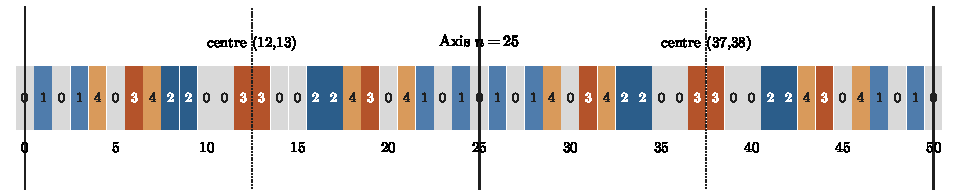
\includegraphics[width=\textwidth]{fig3_palindrome.pdf}
\caption{The sequence $H(n)$ for $n=0,\dots,50$. Solid lines mark the boundaries and the Axis ($n=25$); dotted lines mark the centres of the two inner palindromes, $H(12)=H(13)=3$ and $H(37)=H(38)=3$ (the fifth).}
\label{fig:palindrome}
\end{figure}

\begin{remark}
Because $H$ is even and $25$-periodic, the structure repeats indefinitely. Every multiple of $25/2$ is a centre of symmetry: the Axes are at $n=25j$, and the fifths at the centres are at $n=25j+12.5$. The next palindrome begins at $n=50$, sharing its boundary silence $H(50)=0$ with the previous one.
\end{remark}

% =============================================================================
\section{The counts and the Pythagorean triple}\label{sec:counts}
% =============================================================================

\begin{center}
\begin{tabular}{@{}lcc@{}}
\toprule
 & One Vertebra ($n=0,\dots,24$) & Full Palindrome ($n=0,\dots,50$) \\
\midrule
Silence ($H=0$) & $9=3^{2}$ & $19=2\cdot 9+1$ \\
Unison ($H=1$) & $4=2^{2}$ & $8$ \\
Octave ($H=2$) & $4=2^{2}$ & $8$ \\
Fifth ($H=3$) & $4=2^{2}$ & $8$ \\
Fourth ($H=4$) & $4=2^{2}$ & $8$ \\
\midrule
Total & $25=5^{2}$ & $51=2\cdot5^{2}+1$ \\
\bottomrule
\end{tabular}
\end{center}

\begin{interp}[The Pythagorean Triple, \gr{Ἡ Πυθαγόρειος Τριάς}]
In each Vertebra the silences and the consonances satisfy
\[
  3^{2}+4^{2}=5^{2}:\qquad 9\ \text{(silences)}+16\ \text{(consonances)}=25\ \text{(period)}.
\]
The period $25=5^{2}$ is forced by the denominator $5$ in \eqref{eq:closed}. The count of silences is $5+4$ (Remark after Proposition~\ref{prop:counts}). That these numbers line up with the first Pythagorean triple is a fact; whether it reflects anything deeper is left open (§\ref{sec:discussion}).
\end{interp}

% =============================================================================
\section{The Pentametric–Lucas Theorem}\label{sec:lucas}
% =============================================================================

We use the classical identity \cite{Koshy2001}
\begin{equation}\label{eq:FL}
  L_k^{2}-5F_k^{2}=4(-1)^{k}\qquad(k\ge0).
\end{equation}

\begin{theorem}[The Pentametric–Lucas Theorem]\label{thm:PL}
For every $k\ge0$,
\[
  \Pent(L_k)=F_k^{2},\qquad\text{equivalently}\qquad \sqrt{\Pent(L_k)}=F_k .
\]
\end{theorem}

\begin{proof}
Modulo $5$ the Lucas numbers are periodic with period $4$: $(L_0,L_1,L_2,L_3)\equiv(2,1,3,4)$. Hence $\leg{L_k}=-1,+1,-1,+1$ for $k\equiv0,1,2,3\pmod4$, that is,
\begin{equation}\label{eq:legL}
  \leg{L_k}=-(-1)^{k}.
\end{equation}
In particular $5\nmid L_k$. By \eqref{eq:closed}, \eqref{eq:legL} and \eqref{eq:FL},
\[
  \Pent(L_k)=\frac{L_k^{2}-4(-1)^{k}}{5}=\frac{5F_k^{2}}{5}=F_k^{2}.\qedhere
\]
\end{proof}

\begin{table}[ht]
\centering\small
\caption{Verification of Theorem~\ref{thm:PL} for $k=0,\dots,13$. The identity has also been checked by exact integer arithmetic for all $k\le 59$.}\label{tab:PL}
\begin{tabular}{@{}rrrrrc@{}}
\toprule
$k$ & $n=L_k$ & $\leg{n}$ & $\Pent(n)$ & $\sqrt{\Pent(n)}$ & Fibonacci \\
\midrule
0 & 2 & $-1$ & 0 & 0 & $F_0=0$ \\
1 & 1 & $+1$ & 1 & 1 & $F_1=1$ \\
2 & 3 & $-1$ & 1 & 1 & $F_2=1$ \\
3 & 4 & $+1$ & 4 & 2 & $F_3=2$ \\
4 & 7 & $-1$ & 9 & 3 & $F_4=3$ \\
5 & 11 & $+1$ & 25 & 5 & $F_5=5$ \\
6 & 18 & $-1$ & 64 & 8 & $F_6=8$ \\
7 & 29 & $+1$ & 169 & 13 & $F_7=13$ \\
8 & 47 & $-1$ & 441 & 21 & $F_8=21$ \\
9 & 76 & $+1$ & 1156 & 34 & $F_9=34$ \\
10 & 123 & $-1$ & 3025 & 55 & $F_{10}=55$ \\
11 & 199 & $+1$ & 7921 & 89 & $F_{11}=89$ \\
12 & 322 & $-1$ & 20736 & 144 & $F_{12}=144$ \\
13 & 521 & $+1$ & 54289 & 233 & $F_{13}=233$ \\
\bottomrule
\end{tabular}
\end{table}

The converse also holds: the Lucas numbers are the \emph{only} positions at which $\Pent$ is a perfect square.

\begin{theorem}[Converse]\label{thm:converse}
Let $n\ge1$. Then $\Pent(n)$ is a perfect square if and only if $n$ is a Lucas number. In that case, $n=L_k$ and $\Pent(n)=F_k^{2}$.
\end{theorem}

\begin{proof}
Sufficiency is Theorem~\ref{thm:PL}. Conversely, suppose $\Pent(n)=y^{2}$ with $y\ge0$.
If $5\mid n$, write $n=5j$ with $j\ge1$; then $y^{2}=\Pent(n)=5j^{2}$, which is impossible.
Otherwise $\leg{n}=\varepsilon\in\{\pm1\}$ and $n^{2}=5y^{2}-4\varepsilon$.
If $y=0$, then $n^{2}=4$ and $n=2=L_0$.
If $y\ge1$, then $5y^{2}+4$ or $5y^{2}-4$ is a square. By Gessel's criterion \cite{Gessel1971,Koshy2001}, $y=F_k$ for some $k\ge1$. By \eqref{eq:FL}, $L_k^{2}=5F_k^{2}+4(-1)^{k}$. If $-4\varepsilon=4(-1)^{k}$, then $n=L_k$. If not, then both $5F_k^{2}+4$ and $5F_k^{2}-4$ are squares. Two positive squares differing by $8$ must be $9$ and $1$, so $F_k=1$ and $n\in\{1,3\}=\{L_1,L_2\}$.
\end{proof}

\begin{remark}
Theorem~\ref{thm:converse} corrects an earlier informal statement of the author's: perfect squares among the values of $\Pent$ occur \emph{only} at Lucas positions. At every other $n$, $\Pent(n)$ is an integer within $\tfrac45$ of $n^{2}/5$ but is not a square. A direct check over $1\le n\le 2\times10^{5}$ returns exactly the $26$ Lucas numbers in that range.
\end{remark}


\subsection{The author's conjecture: a simple form at Lucas positions}\label{sec:conjecture}

The Geometric Lucas Meter obtains the distance to the $k$-th centre by a single multiplication, $d_k=L_k\cdot\sqrt{0.1}$. The author conjectured that the area $F_k^{2}$ should be obtainable from $L_k$ in an equally simple way, without the residue machinery of the general formula. The next proposition confirms this conjecture in three forms, and shows exactly how far a single multiplication can go.

\begin{proposition}[Simple forms at Lucas positions]\label{prop:simple}
Let $d_k=L_k\sqrt{0.1}$ be the Lucas-meter distance of the $k$-th centre. Then:
\begin{enumerate}[label=(\alph*),itemsep=3pt]
  \item \emph{Multiply and correct:} $F_k^{2}=\bigl(L_k\sqrt{0.2}\bigr)^{2}-\tfrac45(-1)^{k}=2d_k^{2}-\tfrac45(-1)^{k}$.
  \item \emph{Multiply and round:} for every $k\ge2$, $F_k=\operatorname{round}\bigl(L_k\sqrt{0.2}\bigr)=\operatorname{round}\bigl(\sqrt2\,d_k\bigr)$, and hence $F_k^{2}=\operatorname{round}\bigl(L_k\sqrt{0.2}\bigr)^{2}$.
  \item \emph{Neighbouring centres (exact):} $F_k=\dfrac{L_{k-1}+L_{k+1}}{5}=\sqrt{0.4}\,\bigl(d_{k-1}+d_{k+1}\bigr)$ for $k\ge1$.
  \item \emph{Limit of a pure multiplication:} there is no constant $c$ with $F_k=c\,L_k$ for all $k$, although $F_k/L_k\to\sqrt{0.2}$.
\end{enumerate}
\end{proposition}

\begin{proof}
(a) is \eqref{eq:FL}, using $(L_k\sqrt{0.2})^{2}=L_k^{2}/5=2d_k^{2}$.
(b) With $\psi=(1-\sqrt5)/2$, Binet's formulas $L_k=\varphi^{k}+\psi^{k}$ and $F_k=(\varphi^{k}-\psi^{k})/\sqrt5$ give $L_k\sqrt{0.2}-F_k=2\psi^{k}/\sqrt5$. For $k\ge2$, $|2\psi^{k}/\sqrt5|\le2\psi^{2}/\sqrt5\approx0.342<\tfrac12$.
(c) is the classical identity $L_{k-1}+L_{k+1}=5F_k$ \cite{Koshy2001}, together with $\sqrt{0.1}\,\sqrt{0.4}=0.2$.
(d) $F_1/L_1=1$ while $F_2/L_2=\tfrac13$. The limit follows from (b).
\end{proof}

\begin{remark}
Form (b) answers the conjecture in the sense intended. Up to rounding, the \emph{side} of the $k$-th Fibonacci square is $L_k\cdot\sqrt{0.2}$, just as its distance from $P$ is $L_k\cdot\sqrt{0.1}$. Geometrically, it is $\sqrt2$ times the Lucas-meter distance, i.e.\ the side of the square $S_k$ of Proposition~\ref{prop:geom}. Form (d) shows why rounding, or the exact $\mp\tfrac45$ of form (a), cannot be avoided. That correction is precisely what the Pentametric Formula supplies, since $\Pent(L_k)=(L_k\sqrt{0.2})^{2}+\tfrac45\chi(L_k)$ with $\chi(L_k)=-(-1)^{k}$. Formula (b) was verified by exact high-precision arithmetic for $2\le k<120$; it fails only at $k=0,1$.
\end{remark}

% =============================================================================
\section{The Geometric Lucas Meter (Holden, 1975)}\label{sec:holden}
% =============================================================================

This section states a \emph{classical} result. It is due to H.\,L.~Holden \cite{Holden1975}, was developed further by Hoggatt and Alladi \cite{HoggattAlladi1975}, and was rediscovered by Gardiner \cite{Gardiner1984}. We claim no priority for it. Holden's paper, “Fibonacci Tiles”, does not name the result. In the literature it is described in words, for example “the centres lie on orthogonal lines”. In this paper we refer to it as the \emph{Geometric Lucas Meter} (\gr{Τὸ Γεωμετρικὸν Μέτρον τοῦ Λουκᾶ}), while fully crediting Holden.

\begin{theorem}[Holden 1975 \cite{Holden1975}; see also \cite{HoggattAlladi1975,Gardiner1984}]\label{thm:holden}
Arrange the squares of sides $F_1,F_2,F_3,\dots$ in the standard Fibonacci spiral, and let $C_k$ be the centre of the square of side $F_k$. Then:
\begin{enumerate}[label=(\alph*),itemsep=1pt]
  \item the centres $C_k$ with $k$ odd lie on one straight line, and those with $k$ even lie on a second line perpendicular to the first; the slopes are $3$ and $-\tfrac13$;
  \item if $P$ is the intersection of the two lines, then
  \[
    |C_kP|=\frac{L_k}{\sqrt{10}}=L_k\cdot\sqrt{\tfrac{1}{10}}\qquad(k\ge1).
  \]
\end{enumerate}
\end{theorem}

Holden \cite{Holden1975} proves (a) for an arbitrary generalised Fibonacci sequence $f_k$ and gives the distances as $(f_{k+3}+f_{k-3})/(2\sqrt{10})$. For the Fibonacci numbers, $F_{k+3}+F_{k-3}=2L_k$, which gives (b). Hoggatt and Alladi \cite{HoggattAlladi1975} rederive the centres by generating functions and state the distances as proportional to the Lucas numbers. Gardiner \cite{Gardiner1984} takes the centre of the first square as origin and obtains the two lines explicitly:
\[
  y=3x\quad(\text{odd }k),\qquad 3y=-(x-1)\quad(\text{even }k),\qquad P=\Bigl(\tfrac1{10},\tfrac3{10}\Bigr).
\]
Thus $|C_1P|=\sqrt{0.01+0.09}=\sqrt{0.1}=L_1/\sqrt{10}$. In other words, the Lucas number $L_k$ counts how many units of $\sqrt{0.1}=\sqrt{10}/10$ lie between $P$ and the centre of the $k$-th Fibonacci square.

\begin{remark}[A compact form]
In Gardiner's coordinates, with the spiral turning counter-clockwise as in Figure~\ref{fig:spiral}, put $w=-(1+3i)/10$, so that $|w|=1/\sqrt{10}$. Identifying the plane with $\mathbb{C}$, the centres are
\[
  C_k-P=i^{\,k-1}\,L_k\,w\qquad(k\ge1).
\]
This packages (a) and (b) together: the factor $i^{k-1}$ alternates the centres between the two perpendicular lines, and $L_k|w|$ is the distance. We verified this form by exact rational arithmetic for $k\le16$.
\end{remark}

\begin{figure}[ht]
\centering
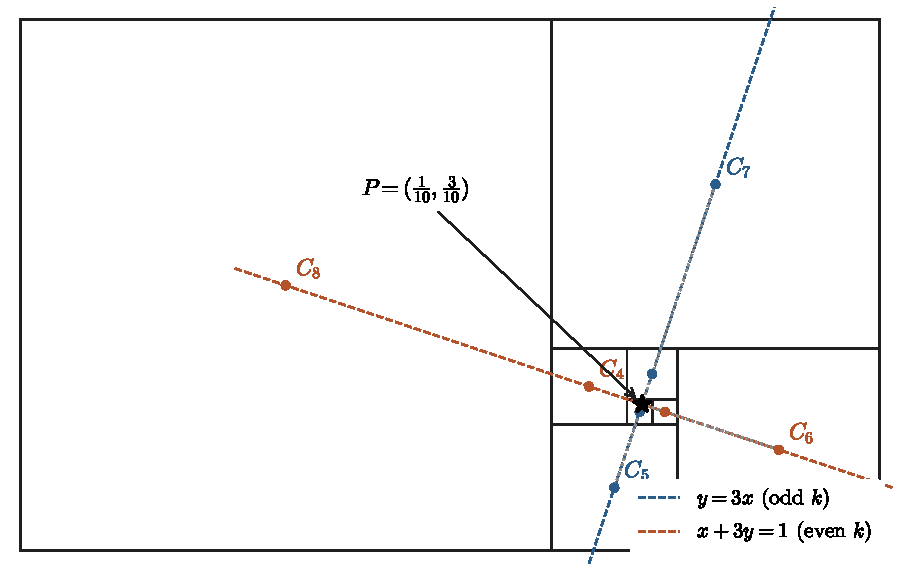
\includegraphics[width=0.92\textwidth]{fig1_spiral.pdf}
\caption{The Geometric Lucas Meter (Holden 1975). Fibonacci squares of sides $1,1,2,3,5,8,13,21$. The centres of odd-indexed squares lie on $y=3x$ and those of even-indexed squares on $x+3y=1$ (Gardiner's coordinates). The lines meet at $P=(\frac1{10},\frac3{10})$, and $|C_kP|=L_k/\sqrt{10}$. Grey dotted segments show $|C_5P|=11/\sqrt{10}$, $|C_6P|=18/\sqrt{10}$ and $|C_7P|=29/\sqrt{10}$.}
\label{fig:spiral}
\end{figure}

\subsection{Correspondence with the Pentametric–Lucas Theorem}

\begin{center}
\begin{tabular}{@{}lll@{}}
\toprule
 & Pentametric–Lucas Theorem (new) & Geometric Lucas Meter (Holden 1975) \\
\midrule
Statement & $\Pent(L_k)=F_k^{2}$ & $|C_kP|=L_k\cdot\sqrt{1/10}$ \\
Role of $L_k$ & argument giving the \emph{area} & multiplier giving the \emph{position} \\
Object & the Fibonacci square & the centre of that square \\
\bottomrule
\end{tabular}
\end{center}

\noindent Together, the two statements form a complete correspondence: the Lucas number $L_k$ simultaneously indexes the $k$-th Fibonacci square (via its area) and locates its centre (via its distance from $P$).

\subsection{A geometric reading of \texorpdfstring{$\Pent$}{P} in the Fibonacci tiling}\label{sec:geom-new}

The two statements are linked by a single geometric construction. This construction, and the identities below, are the author's contribution. They correspond to the “$\pm0.8$” and “$\pm2\pi/5$” constructions in the accompanying GeoGebra files.

\begin{proposition}[Square and circle identities]\label{prop:geom}
Let $Q_k$ be the Fibonacci square of side $F_k$ with centre $C_k$. Let $\Gamma_k$ be the circle with centre $C_k$ passing through $P$, and let $S_k$ be the square inscribed in $\Gamma_k$ with a vertex at $P$. Let $\Omega_k$ be the circumcircle of $Q_k$. Then for every $k\ge1$:
\begin{enumerate}[label=(\alph*),itemsep=1pt]
  \item $S_k$ has side $L_k/\sqrt5=L_k\sqrt{0.2}$ and
  \[
    \operatorname{area}(S_k)=\frac{L_k^{2}}{5}=F_k^{2}+\frac45(-1)^{k}=\operatorname{area}(Q_k)\pm\frac45;
  \]
  \item $\operatorname{area}(\Gamma_k)-\operatorname{area}(\Omega_k)=\dfrac{2\pi}{5}(-1)^{k}$;
  \item $\Pent$ removes the discrepancy in (a): $\Pent(L_k)=\operatorname{area}(S_k)-\frac45(-1)^{k}=\operatorname{area}(Q_k)$.
\end{enumerate}
\end{proposition}

\begin{proof}
By Theorem~\ref{thm:holden}, $\Gamma_k$ has radius $r_k=L_k/\sqrt{10}$. The inscribed square has diagonal $2r_k$ and side $\sqrt2\,r_k=L_k/\sqrt5$, so its area is $L_k^{2}/5$. Part (a) follows from \eqref{eq:FL}. For (b), $\Omega_k$ has radius $F_k/\sqrt2$, so the difference of areas is $\pi\bigl(L_k^{2}/10-F_k^{2}/2\bigr)=\tfrac{\pi}{10}\bigl(L_k^{2}-5F_k^{2}\bigr)=\tfrac{2\pi}{5}(-1)^{k}$. Part (c) is \eqref{eq:closed} combined with \eqref{eq:legL}.
\end{proof}

\begin{figure}[ht]
\centering
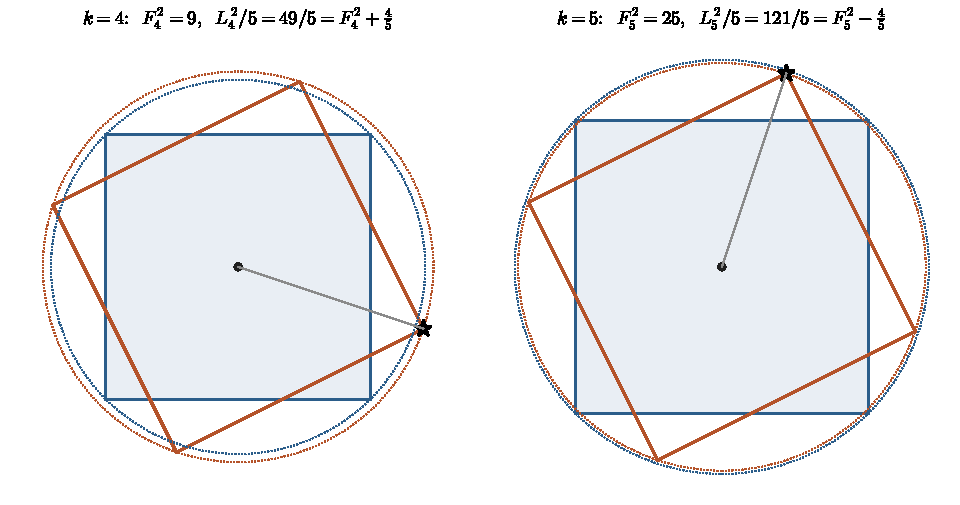
\includegraphics[width=\textwidth]{fig2_area.pdf}
\caption{Proposition~\ref{prop:geom} for $k=4$ and $k=5$. Shaded: the Fibonacci square $Q_k$. Red: the square $S_k$ centred at $C_k$ with a vertex at $P$ (star); its area is $L_k^{2}/5=F_k^{2}\pm\frac45$. Dotted: the circles $\Gamma_k$ (through $P$) and $\Omega_k$ (circumcircle of $Q_k$), whose areas differ by $\pm\frac{2\pi}{5}$.}
\label{fig:area}
\end{figure}


\subsection{The angles of the construction}\label{sec:angles}

The author's angle tables (\texttt{Angles.xlsx}) tabulate $\arctan$ of the ratios $1/3$, $1/2$, $3/4$, $4/3$ and others, together with their sines, cosines and doubles. Two of these angles govern the geometry above.

\begin{proposition}[The two angles]\label{prop:angles}
Let $\theta_1=\arctan\frac13$ and $\theta_2=\arctan\frac12$. Then:
\begin{enumerate}[label=(\alph*),itemsep=2pt]
  \item $\sin\theta_1=\sqrt{0.1}$ and $\sin\theta_2=\sqrt{0.2}$. These are the unit of the Geometric Lucas Meter and the side unit $n\sqrt{0.2}$ of Proposition~\ref{prop:defects}.
  \item Holden's lines $y=3x$ and $x+3y=1$ make the angle $\theta_1$ with the vertical and horizontal axes of the tiling, respectively. The vector from $C_1$ to $P$ is $\sqrt{0.1}\,(\sin\theta_1,\cos\theta_1)$.
  \item For every $k\ge1$, the sides of the square $S_k$ of Proposition~\ref{prop:geom} have slopes $\frac12$ and $-2$, that is, they are inclined at $\theta_2$ to the axes of the tiling.
  \item $\theta_1+\theta_2=\frac{\pi}{4}$, and $\tan2\theta_1=\frac34$, $\tan2\theta_2=\frac43$. Thus $2\theta_1$ and $2\theta_2$ are the two acute angles of the $3$–$4$–$5$ right triangle, and $2\theta_1+2\theta_2=\frac{\pi}{2}$.
\end{enumerate}
\end{proposition}

\begin{proof}
(a) $\sin\arctan t=t/\sqrt{1+t^{2}}$, which gives $\frac{1/3}{\sqrt{10}/3}=\frac1{\sqrt{10}}$ and $\frac{1/2}{\sqrt5/2}=\frac1{\sqrt5}$.
(b) This is immediate from the slopes $3$ and $-\frac13$ and from $P-C_1=(\frac1{10},\frac3{10})$.
(c) In the notation of the remark following Theorem~\ref{thm:holden}, $P-C_k=-i^{k-1}L_kw$, whose direction is $\arg(1+3i)+(k-1)\frac{\pi}{2}=\frac{\pi}{2}-\theta_1+(k-1)\frac{\pi}{2}$. A side of the square inscribed in $\Gamma_k$ with a vertex at $P$ is $(i-1)(P-C_k)$, which turns this direction by $\frac{3\pi}{4}$. Modulo $\frac{\pi}{2}$, the side direction is therefore $\frac{\pi}{4}-\theta_1=\theta_2$.
(d) $\tan(\theta_1+\theta_2)=\frac{1/3+1/2}{1-1/6}=1$ (Euler's arctangent identity). $\tan2\theta_1=\frac{2/3}{1-1/9}=\frac34$ and $\tan2\theta_2=\frac{1}{1-1/4}=\frac43$.
\end{proof}

\begin{interp}
Proposition~\ref{prop:angles}(d) is a \emph{geometric} appearance of the triple $3^{2}+4^{2}=5^{2}$ in the Fibonacci tiling. It is independent of the count $9+16=25$ of §\ref{sec:counts}. The orientation of Holden's lines ($\theta_1$) and the orientation of the squares $S_k$ ($\theta_2$) are the half-angles of the $3$–$4$–$5$ triangle.
\end{interp}

% =============================================================================
\section{The complete nomenclature}\label{sec:nomenclature}
% =============================================================================

\begin{center}
\small
\renewcommand{\arraystretch}{1.25}
\begin{tabularx}{\textwidth}{@{}>{\raggedright\arraybackslash}p{4.1cm}>{\raggedright\arraybackslash}p{3.6cm}>{\raggedright\arraybackslash}p{3.4cm}X@{}}
\toprule
Greek & Transliteration & English & Role \\
\midrule
\gr{Ὁ Πενταμετρικὸς Κύκλος} & Ho Pentametrikos Kyklos & The Pentametric Cycle & Whole system \\
\gr{Ὁ Πενταμετρικὸς Παλίνδρομος} & Ho Pentametrikos Palindromos & The Pentametric Palindrome & Full palindrome (51) \\
\gr{Ὁ Πεντάμετρος Σπόνδυλος} & Ho Pentametros Spondylos & The Pentametric Vertebra & Fundamental period (25) \\
\gr{Αἱ Εἴκοσι Τέσσαρες Μεταβάσεις} & Hai Eikosi Tessares Metabaseis & The Twenty-Four Transitions & Transitions (24) \\
\gr{Ὁ Ἄξων} & Ho Axōn & The Axis & Mirror point ($n=25$) \\
\gr{Τὸ Τετράγωνον Σπέρμα} & To Tetragōnon Sperma & The Square Seed & Consonance skeleton (16) \\
\gr{Ἡ Τριαδικὴ Σιγή} & Hē Triadikē Sigē & The Triadic Silence & Silence skeleton (9) \\
\gr{Αἱ Τέσσαρες Συμφωνίαι} & Hai Tessares Symphōniai & The Four Consonances & The intervals (4) \\
\gr{Ἡ Πυθαγόρειος Τριάς} & Hē Pythagoreios Trias & The Pythagorean Triple & Structural identity \\
\gr{Ὁ Πενταμετρικὸς Τύπος} & Ho Pentametrikos Typos & The Pentametric Formula & Generator ($\Pent$) \\
\gr{Ὁ Διαστηματικὸς Χάρτης} & Ho Diastēmatikos Chartēs & The Interval Map & Ratio mapper $C(m)$ \\
\gr{Ὁ Ἁρμονικὸς Κανών} & Ho Harmonikos Kanōn & The Harmonic Canon & Alternative name of $C(m)$ \\
\gr{Τὸ Γεωμετρικὸν Μέτρον τοῦ Λουκᾶ} & To Geōmetrikon Metron tou Louka & The Geometric Lucas Meter & Distance to square centres (Holden 1975) \\
\bottomrule
\end{tabularx}
\end{center}

% =============================================================================
\section{The structure diagram}\label{sec:diagram}
% =============================================================================

\begin{center}
\small
\begin{forest}
  for tree={
    font=\small,
    grow'=0,
    folder,
    folder indent=0.6em,
    edge={line width=0.5pt},
    s sep=2pt,
    inner ysep=1.5pt,
  }
  [{\gr{Ὁ Πενταμετρικὸς Κύκλος} (The Pentametric Cycle)}
    [{\gr{Ὁ Πενταμετρικὸς Παλίνδρομος} (The Pentametric Palindrome) — 51 terms}
      [{Part 1: \gr{Ὁ Πεντάμετρος Σπόνδυλος} (The Pentametric Vertebra) — $25=5^{2}$}
        [{\gr{Τὸ Τετράγωνον Σπέρμα} (The Square Seed) — $16=4^{2}$}
          [{\gr{Αἱ Τέσσαρες Συμφωνίαι} (The Four Consonances) — $4=2^{2}$ each}]
        ]
        [{\gr{Ἡ Τριαδικὴ Σιγή} (The Triadic Silence) — $9=3^{2}$}]
        [{\gr{Αἱ Εἴκοσι Τέσσαρες Μεταβάσεις} (The Twenty-Four Transitions) — $24=4!$}]
      ]
      [{\gr{Ὁ Ἄξων} (The Axis) — position $25$, self-mirroring}]
      [{Part 2: \gr{Ὁ Πεντάμετρος Σπόνδυλος} reversed — $25=5^{2}$}]
    ]
    [{\gr{Ὁ Πενταμετρικὸς Τύπος} (The Pentametric Formula) — $\Pent(n)$}
      [{\gr{Ὁ Διαστηματικὸς Χάρτης} (The Interval Map) — $C(m)=\leg{n}$}]
      [{\gr{Ἡ Σχέσις} Fibonacci–Lucas (The Fibonacci–Lucas Relation) — $\Pent(L_k)=F_k^{2}$}]
    ]
    [{\gr{Ἡ Πυθαγόρειος Τριάς} (The Pythagorean Triple) — $3^{2}+4^{2}=5^{2}$}]
    [{\gr{Τὸ Γεωμετρικὸν Μέτρον τοῦ Λουκᾶ} (The Geometric Lucas Meter, Holden 1975) — $L_k\cdot\sqrt{1/10}$}]
  ]
\end{forest}
\end{center}

% =============================================================================
\section{Musical significance}\label{sec:music}
% =============================================================================

This section separates two kinds of statement. The first subsection lists facts that follow by proof once the ratio rule $\rho(H)=H:(H-1)$ of Definition~\ref{def:ratio} is fixed; they are computed, not interpreted. The second lists readings that connect the cycle to the Pythagorean tradition; they are interpretive and are not part of the mathematical claims.

\subsection{Derived musical facts}

\begin{enumerate}[itemsep=2pt]
  \item \emph{All four consonances, in equal number.} The ratios $\rho(H(n))$ take exactly the values $1:1$, $2:1$, $3:2$ and $4:3$, each four times per Vertebra and eight times per Palindrome, with nine (respectively nineteen) silences (Propositions~\ref{prop:counts} and~\ref{prop:palindrome}).
  \item \emph{The consonances are the tetractys ratios.} For $H=2,3,4$ the single rule $H:(H-1)$ yields $2:1$, $3:2$, $4:3$: the octave, fifth and fourth, i.e.\ exactly the ratios of consecutive members of $1,2,3,4$ \cite{Levin1994,Bower1989}.
  \item \emph{The fifth at the centre.} The two inner palindromes are centred on the pairs $H(12)=H(13)=3$ and $H(37)=H(38)=3$, so the interval at each centre is the fifth $3:2$ (Proposition~\ref{prop:period}).
  \item \emph{Symmetric distribution.} The interval sequence $n\mapsto\rho(H(n))$ is $25$-periodic and mirrors at every Axis $n=25j$ (Propositions~\ref{prop:period} and~\ref{prop:palindrome}).
  \item \emph{A computed annotation.} The musical annotation $\note(n)=\rho(H(n))$ is determined at every position $n$ by the seven-step chain of §\ref{sec:derivation}.
\end{enumerate}

\subsection{Interpretive readings}

\begin{enumerate}[itemsep=2pt,resume]
  \item The doubling $2\Pent$ is read as the diapason (octave), the fundamental musical operation; halving then recovers the consonance indicator.
  \item In the Pythagorean tradition, the fifth is the generator of the scale: Pythagorean tuning is built by stacking fifths and reducing by octaves \cite{Barker1989}. That the fifth occupies the centre of the palindrome (item~3) is therefore suggestive.
  \item The period splits as $3^{2}+4^{2}=5^{2}$ (silences, consonances, period), recalling the first Pythagorean triple; the same triple appears geometrically in the angles of the construction (Proposition~\ref{prop:angles}).
  \item The $24$ transitions of a Vertebra match in number, though not one-to-one (§\ref{sec:dual}), the $4!$ orderings of the four consonances.
\end{enumerate}

% =============================================================================
\section{Mathematical significance}\label{sec:math}
% =============================================================================

\begin{enumerate}[itemsep=2pt]
  \item The Pentametric Formula has the closed form $\Pent(n)=(n^{2}+4\leg{n})/5$. It is the integer obtained by shifting $n^{2}/5$ by $\pm\tfrac45$ according to the quadratic character of $n$ modulo $5$ (Lemma~\ref{lem:legendre}).
  \item The ten forms (F1)–(F10) of $\Pent$ (Theorem~\ref{thm:family}) reach the same areas through digits, floors, a quintic polynomial, a Gauss sum, golden-ratio rotations and pentagonal angles. They are unified by the quadratic character modulo~$5$.
  \item The cycle is nested: Palindrome ($51$) $\supset$ Vertebra ($25$) $\supset$ Square Seed ($16$) $\supset$ each Consonance ($4$). The counts $25,16,9,4$ are $5^{2},4^{2},3^{2},2^{2}$.
  \item The consonance sequence $H$ is even and has minimal period $25$, so it is palindromic about every multiple of $25/2$ (Proposition~\ref{prop:period}).
  \item The Pentametric–Lucas Theorem $\Pent(L_k)=F_k^{2}$ holds for all $k\ge0$, and conversely the perfect-square values of $\Pent$ occur exactly at the Lucas numbers (Theorems~\ref{thm:PL}–\ref{thm:converse}). At Lucas positions the side is $\operatorname{round}(L_k\sqrt{0.2})$, mirroring the distance $L_k\sqrt{0.1}$ (Proposition~\ref{prop:simple}).
  \item In the Fibonacci tiling, the Lucas number $L_k$ both returns the area of the $k$-th square through $\Pent$ and measures the distance $L_k\sqrt{1/10}$ to its centre (Holden 1975). The square and circle identities of Proposition~\ref{prop:geom} make the correction term $\pm\tfrac45$ of $\Pent$ visible as a geometric area.
  \item To the best of our knowledge, neither the sequence $\Pent(n)$ ($0,1,0,1,4,5,8,9,12,17,\dots$) nor the sequence $H(n)$ appears in the On-Line Encyclopedia of Integer Sequences \cite{OEIS} (searched October 2026).
\end{enumerate}

% =============================================================================
\section{Discussion}\label{sec:discussion}
% =============================================================================

The Pentametric Cycle sits at the intersection of elementary number theory, the geometry of the Fibonacci tiling, and the Pythagorean theory of consonance. Its connections to classical results are the following.

\begin{itemize}[itemsep=2pt]
  \item The Fibonacci–Lucas identity $F_k^{2}=(L_k^{2}-4(-1)^{k})/5$ is the identity underlying Theorem~\ref{thm:PL}. The Pentametric Formula extends its right-hand side from the Lucas numbers to all integers by replacing $-(-1)^{k}$ with the Legendre symbol $\leg{n}$, which agrees with it on Lucas numbers by \eqref{eq:legL}.
  \item Gessel's test for Fibonacci numbers \cite{Gessel1971} is equivalent to the statement that the square values of $\Pent$ occur exactly at the Lucas numbers (Theorem~\ref{thm:converse}).
  \item Holden \cite{Holden1975} showed that the centres of spiralling Fibonacci squares lie on orthogonal lines at distances proportional to the Lucas numbers. This geometric result complements the Pentametric–Lucas Theorem: the Lucas number simultaneously indexes the square (via area) and locates its centre (via distance). Proposition~\ref{prop:geom} shows that the two are linked by a single construction.
  \item The cosine and golden-rotation forms (F8)–(F9) are instances of the quadratic Gauss sum modulo $5$, $\cos\frac{2\pi n}{5}-\cos\frac{4\pi n}{5}=\frac{\sqrt5}{2}\leg{n}$ \cite{IrelandRosen1990}. This explains why the angles $72^\circ$ and $144^\circ$ of the regular pentagon appear in the author's constructions.
  \item Holden's lines are inclined at $\arctan\frac13$, and the squares $S_k$ at $\arctan\frac12$. Their doubles are the acute angles of the $3$–$4$–$5$ triangle (Proposition~\ref{prop:angles}).
  \item The doubling $2\Pent$ is the musical octave, and the halving recovers the consonances. The split $9+16=25$ recalls the triple $3^{2}+4^{2}=5^{2}$.
\end{itemize}

\paragraph{Open questions.}
\begin{enumerate}[itemsep=2pt]
  \item \emph{Other moduli.} Replacing $5$ by another prime $p$ gives the analogous construction $\Pent_p(n)=(n^{2}+c\,(n/p))/p$. For which $p$ and $c$ is it integer-valued? Does the analogous consonance sequence have period $p^{2}$, and does its zero count again split as a sum of two squares?
  \item \emph{Other recurrences.} Holden's lines exist for every generalised Fibonacci sequence \cite{Holden1975,HoggattAlladi1975}. Is there a Pentametric formula whose square values are exactly $f_k^{2}$ at the companion sequence for a generalised Fibonacci sequence $f_k$, or for Pell and Pell–Lucas numbers?
  \item \emph{Other triples.} Is there a companion cycle whose counts realise another Pythagorean triple, such as $5^{2}+12^{2}=13^{2}$?
  \item \emph{Continued fractions.} $\Pent(n)$ is determined by $n^{2}/5$ and the quadratic character of $n$ modulo $5$. What is the precise connection to the continued fraction expansion of $\sqrt5$, and to rational approximations of $\varphi$?
  \item \emph{The transitions.} Does the multiset of the $24$ transitions, with its $17$ distinct pairs, have an intrinsic combinatorial description?
\end{enumerate}

% =============================================================================
\section{Conclusion}\label{sec:conclusion}
% =============================================================================

The Pentametric Cycle is a family of equivalent formulas generating a nested palindrome that encodes the four Pythagorean consonances. We have shown that the Pentametric Formula equals $(n^{2}+4\leg{n})/5$, that its consonance sequence has period $25$ with the counts $9+16=25$, and that it satisfies the Pentametric–Lucas Theorem $\Pent(L_k)=F_k^{2}$ together with its converse. Holden's classical result of 1975 on Fibonacci tiles provides a complementary geometric perspective, in which the Lucas number simultaneously indexes the square and locates its centre. The square and circle identities of Proposition~\ref{prop:geom} join the two perspectives. The formula and its nomenclature offer a new perspective on the Pythagorean tradition, and open several directions for further research.

% =============================================================================
\section*{Acknowledgements}
\addcontentsline{toc}{section}{Acknowledgements}
% =============================================================================

The geometric result on the centres of Fibonacci squares is due to H.\,L.~Holden (1975); the connection to the Pentametric Cycle, the Pentametric–Lucas Theorem and its converse, and the square and circle identities of Proposition~\ref{prop:geom} are the author's contribution.

The author used an AI assistant (Claude, developed by Anthropic) to help write the manuscript and to check the proofs and numerical results independently. The author is responsible for the content of the paper.

\section*{Data and materials availability}
\addcontentsline{toc}{section}{Data and materials availability}

The GeoGebra constructions, spreadsheets and images that accompany this paper are available in the author's repository \emph{The Pentametric Cycle}, \url{https://github.com/lluisgarcia/The-Pentametric-Cycle}. All numerical statements in this paper were verified independently by exact integer and rational arithmetic.

% =============================================================================
\begin{thebibliography}{99}
\addcontentsline{toc}{section}{References}
% =============================================================================

\bibitem{Holden1975}
H.\,L.~Holden, Fibonacci tiles, \emph{The Fibonacci Quarterly} \textbf{13}(1) (February 1975), 45--49.

\bibitem{HoggattAlladi1975}
V.\,E.~Hoggatt,~Jr.\ and K.~Alladi, Generalized Fibonacci tiling, \emph{The Fibonacci Quarterly} \textbf{13}(2) (April 1975), 137--144.

\bibitem{Gardiner1984}
T.~Gardiner, 68.15 The Fibonacci spiral, \emph{The Mathematical Gazette} \textbf{68}(444) (June 1984), 120. \href{https://doi.org/10.2307/3615922}{doi:10.2307/3615922}.

\bibitem{Gessel1971}
I.~Gessel, Problem H-187, \emph{The Fibonacci Quarterly} \textbf{9}(5) (December 1971), 512.

\bibitem{Koshy2001}
T.~Koshy, \emph{Fibonacci and Lucas Numbers with Applications}, Wiley-Interscience, New York, 2001.

\bibitem{Barker1989}
A.~Barker, \emph{Greek Musical Writings, Vol.~II: Harmonic and Acoustic Theory}, Cambridge University Press, Cambridge, 1989.

\bibitem{Levin1994}
F.\,R.~Levin, \emph{The Manual of Harmonics of Nicomachus the Pythagorean}, Phanes Press, Grand Rapids, 1994.

\bibitem{Bower1989}
Boethius, \emph{Fundamentals of Music}, transl.\ C.\,M.~Bower, ed.\ C.\,V.~Palisca, Yale University Press, New Haven, 1989.

\bibitem{Griffiths2018}
D.\,J.~Griffiths and D.\,F.~Schroeter, \emph{Introduction to Quantum Mechanics}, 3rd ed., Cambridge University Press, Cambridge, 2018.

\bibitem{IrelandRosen1990}
K.~Ireland and M.~Rosen, \emph{A Classical Introduction to Modern Number Theory}, 2nd ed., Graduate Texts in Mathematics~84, Springer, New York, 1990.

\bibitem{OEIS}
OEIS Foundation Inc., \emph{The On-Line Encyclopedia of Integer Sequences}, \url{https://oeis.org}.

\end{thebibliography}

% =============================================================================
\appendix
\section{Computational verification}\label{app:verify}
% =============================================================================

All claims were checked with exact arithmetic (Python \texttt{fractions}):
\begin{itemize}[itemsep=1pt]
  \item Definition~\ref{def:P} and the closed form \eqref{eq:closed} agree, and $\Pent(n)\in\Z$, for $0\le n<10^{4}$; the residue $m$ takes only the values $0,4,6$.
  \item $H$ has minimal period $25$; the blocks $H(1..24)$, $H(0..25)$ and $H(0..50)$ are palindromes, while $H(0..24)$ is not.
  \item Counts: $\{0{:}\,9;\ 1,2,3,4{:}\,4\}$ on $0..24$; $\{0{:}\,19;\ 1,2,3,4{:}\,8\}$ on $0..50$.
  \item $\Pent(L_k)=F_k^{2}$ for $0\le k\le 59$; for $1\le n\le 2\times10^{5}$, $\Pent(n)$ is a square exactly at the $26$ Lucas numbers in that range.
  \item The ten forms (F1)–(F10) of Theorem~\ref{thm:family}, the side-length correction of Corollary~\ref{cor:side} and both defects of Proposition~\ref{prop:defects} agree with $\Pent(n)$ for $0\le n<3000$ (exactly for the rational forms, to $10^{-6}$ relative error for the trigonometric ones). This was checked independently of, and in agreement with, the author's spreadsheets.
  \item The Fibonacci spiral was built with exact rational coordinates for $k\le16$. The odd and even centres are collinear on $y=3x$ and $x+3y=1$; $10\,|C_kP|^{2}=L_k^{2}$; and $C_k-P=i^{k-1}L_kw$.
\end{itemize}

\end{document}
